\documentclass[12pt,spanish,fleqn,openany,letterpaper,pagesize]{scrbook}
\usepackage[utf8]{inputenc}
\usepackage[spanish]{babel}
\usepackage[colorlinks,urlcolor=blue,citecolor=black]{hyperref}
\usepackage{fancyhdr}
\usepackage{epsfig}
\usepackage{epic}
\usepackage{eepic}
\usepackage{amsmath}
\usepackage{threeparttable}
\usepackage{amscd}
\usepackage{here}
\usepackage{graphicx}
\usepackage{lscape}
\usepackage{tabularx}
\usepackage{subfigure}
\usepackage{longtable}
\usepackage{apacite}
\usepackage{rotating}
\usepackage{todonotes}
\usepackage{multirow}
\usepackage{booktabs}
\usepackage{url}
\usepackage{arydshln}
\usepackage{color,soul}
\usepackage[nottoc,numbib]{tocbibind}
\usepackage{rotating}
\usepackage[toc]{glossaries}
\makeglossaries
\renewcommand{\theequation}{\thechapter-\arabic{equation}}
\renewcommand{\thefigure}{\textbf{\thechapter-\arabic{figure}}}
\renewcommand{\thetable}{\textbf{\thechapter-\arabic{table}}}
\pagestyle{fancyplain}%\addtolength{\headwidth}{\marginparwidth}
\textheight22.5cm \topmargin0cm \textwidth16.5cm
\oddsidemargin0.5cm \evensidemargin-0.5cm%
\renewcommand{\chaptermark}[1]{\markboth{\thechapter\; #1}{}}
\renewcommand{\sectionmark}[1]{\markright{\thesection\; #1}}
\lhead[\fancyplain{}{\thepage}]{\fancyplain{}{\rightmark}}
\rhead[\fancyplain{}{\leftmark}]{\fancyplain{}{\thepage}}
\fancyfoot{}
\thispagestyle{fancy}%

\addtolength{\headwidth}{0cm}
\unitlength1mm %Define la unidad LE para Figuras
\mathindent0cm %Define la distancia de las formulas al texto,  fleqn las descentra
\marginparwidth0cm
\parindent0cm %Define la distancia de la primera linea de un parrafo a la margen


\newcommand{\PreserveBackslash}[1]{\let\temp=\\#1\let\\=\temp}
\let\PBS=\PreserveBackslash
\newglossaryentry{docker_compose}{name={docker-compose},description={A strange animal}}

\newglossaryentry{vagrant}{name={Vagrant},description={Un sistema open source para la construción y mantenimiento de ambientes desarrollo portables a través del uso de diferentes Hypervisors como Virtualbox \url{http://www.virtualbox.com}}}

\newglossaryentry{script}{name={script},description={Que es un script}}

\newglossaryentry{ssh}{name={SSH},description={Que es un script}}
\newglossaryentry{ansible}{name={Ansible},description={Que es un script}}

\renewcommand{\baselinestretch}{1.1}
\newcommand{\arr}[1]{\raisebox{1.5ex}[0cm][0cm]{#1}}

\hypersetup{
    colorlinks=true,
    linkcolor=blue,
    filecolor=magenta,      
    urlcolor=cyan,
    pdftitle={SMMD},
    bookmarks=true,
    pdfpagemode=FullScreen,
}

\begin{document}
\pagenumbering{roman}
\include{titulo/titulo}
\renewcommand{\tablename}{\textbf{Tabla}}
\renewcommand{\figurename}{\textbf{Figura}}
\renewcommand{\listtablename}{Lista de Tablas}
\renewcommand{\listfigurename}{Lista de Figuras}
\renewcommand{\contentsname}{Contenido}
\tableofcontents
\listoffigures
\listoftables
\pagenumbering{arabic}
\chapter{Introducción}
\section{¿Qué es un centro de computación de alto desempeño?}

El término ``Computación de Alto desempeño'' hace referencia a la distribución de la carga computacional para la solución de problemas científicos haciendo uso de tecnologías que implementan la distribución de carga en un conjunto de recursos computacionales coordinados llamados clusters. De acuerdo a \cite{insidehpc} la computación de alto desempeño generalmente se refiere a la práctica de agregar poder computacional de tal forma que este entrega mucho más rendimiento que cualquier recurso de computo individual con el propósito de solucionar problemas en diversos campos como la ingeniería, la ciencias básicas y la economía.
\newline
\newline
Como cualquier recurso computacional un sistema de computación de alto desempeño debe abordarse desde sus componentes más básicos, en escencia se puede comprender desde los componentes de cualquier sistema de computo en términos de sus elementos de hardware tales como memoria, procesador, almacenamiento y sus elementos de software tales como sistema operativo y aplicaciones de usuario.
Partiendo desde estos componentes básicos, podemos afirmar que un centro de computación de alto desempeño es la suma de todos los recursos de hardware de diferentes nodos los cuales a través de un circuito lógico construido por el sistema operativo, la comunicación en red y el software componen un único sistema multipropósito, en el cual se pueden procesar grandes volúmenes de información, ejecutar diversos algoritmos y procesamiento de cálculos con gran velocidad y alto rendimiento.
\\\\
Para dar idea de la magnitud de recursos de hardware que se pueden conformar en un centro de computo de alto desempeño, para Noviembre de 2018, en los Estados Unidos la supercomputadora número 1 Power System AC922 de IBM tiene 2,397,824 núcleos de procesador y una memoria RAM de 2,801,664 Gigabytes alcanzando un máximo teórico de 200,795 Tera flops por segundo \cite{top500_supercomputer_sites_2019} lo que da cuenta del poder computacional con el que se pueden solucionar diversos problemas de la ciencia y la ingeniería.

\newpage

\section{¿Por que es importante monitorear el desempeño en centros de cómputo de alto desempeño?}

Los centros de cómputo de alto desempeño son recursos totalmente necesarios en entidades académicas, investigativas o comerciales, que requieran el almacenamiento y procesamiento de altos volúmenes de datos que exijan tareas intensivas y complejas.  El potencial de cada uno de esos centros de cómputo se basa en las especificaciones y configuración de su infraestructura y en el buen uso que se haga de ésta por parte de las aplicaciones que se ejecutan allí. La gestión y administración de un centro de cómputo de alto rendimiento y la alta eficiencia con la cual las aplicaciones sacan provechos de la infraestructura depende en gran parte del control continuo que se tenga sobre el uso de los recursos con los cuales se cuenta, sin embargo este es uno de los problemas en los cuales los investigadores invierten mucho tiempo para encontrar herramientas de software que permitan la obtención de métricas básicas, las herramientas usadas son diversas y dependen de las necesidades del actor, de la infraestructura, de la tecnología y del software. Esto conlleva a que tanto la administración del centro como cada uno de los proyectos ejecutados en él instalen, configuren y en algunos casos desarrollen herramientas específicas de monitoreo de métricas de desempeño agregando esfuerzo y tiempo que podría ser utilizado en la resolución del problema científico, ejemplo evidente en el caso de los proyectos de bioinformática desarrollados en el convenio del GICOGE con el Instituto de Genética de la Universidad Nacional.


\section{Objetivos}
El objeto del presente proyecto es el diseño, implementación y evaluación de un sistema modular de adquisición, gestión y visualización web de métricas de rendimiento para centros de cómputo de alto desempeño. Métricas tales como: uso de CPU, utilización de memoria RAM, espacio en disco, conteo de procesos, tráfico de red, operaciones de I/O en disco, cantidad de hilos, uso de memoria en GPU serán gestionadas mediante un motor de búsqueda como Elasticsearch y serán visualizadas haciendo uso de herramientas como Kibana. El sistema  tendrá un diseño de naturaleza modular con el fin de adaptarse a las diferentes naturalezas de los centros de cómputo de alto desempeño y a su continuo crecimiento e inclusión de nuevas tecnologías. La implementación realizada será un caso de estudio específicamente para el CECAD.
Crear un modelo de sistema modular para la adquisición, gestión y visualización web para métricas de desempeño en centros de cómputo de alto rendimiento.
Construir una implementación del sistema modelado para el caso específico del CECAD.
Evaluar el sistema implementado mediante su uso por parte de los proyectos vigentes en el CECAD.
Generar proyecciones y prospectivas de uso e innovación (mejoras, optimización y transformación) del sistema.

\section{Pregunta problema e hipotésis de la investigación}
¿Qué especificaciones debe cumplir un sistema modular de adquisición, gestión y visualización web de métricas de desempeño para centros de cómputo de alto rendimiento?
\\\\
Un sistema modular de adquisición, gestión y visualización, debe ser capaz de utilizarse de una manera sencilla y amigable, en donde el investigador no tenga la necesidad de invertir el tiempo en encontrar la combinación de herramientas y tecnologías que le permitan conocer métricas básicas necesarias para la medición y comparación de rendimiento en el procesamiento de datos y ejecución de algoritmos. \\El sistema debe ser capaz de entregar métricas básicas tales como el uso de procesador, memoria, almacenamiento en una interfaz sencilla y de fácil acceso.
Debido los interes particulares entre quienes administran los centros de cómputo de alto rendimiento y quienes hacen uso de ellos, es necesario que la herramienta de adquisición, gestión y visualización sea independiente de tal manera que se pueda instalar, configurar y ejecutar con los ajustes que requiera el investigador sin la necesidad de interefir con el software de administración del centro computo, permitiendole al investigador trabajar de manera autonoma y aislada dando espacio para que diversos proyectos se ejecuten en el mismo centro de computo sin interferencia alguna.

\newpage

\section{Como se organiza esta investigación}

El proyecto esta planteado en tres fases principales las cuales son: Diseño, Implemetación y Evaluación, dichas fases están organizadas en cápitulos donde se describen las actividades y los modelos que componen el sistema de monitoreo y administración de métricas de desempeño.

\begin{table}[h]
\centering
\begin{tabular}{c m{10cm} c}
\toprule
\textbf{Fase} & \centering{\textbf{Descripción}} & \textbf{Capítulo}\\[3ex]
\midrule
\multirow{3}{*}{Diseño} & Estado del arte sobre monitoreo en centros de cómputo de alto desempeño & 1\\
 & Definición de tecnologías y metodología  & 2\\
 & Diseño de la arquitectura general del sistema. & 3\\
\hdashline
\multirow{3}{*}{Implementación} & Configuración del entorno & 4 \\
 & Instalación &  4.1\\
 & Ejecución de módulos y verificación & \\
\hdashline
\multirow{3}{*}{Evaluación} & Verificación del sistema y métricas & \multirow{3}{*}{1}\\
 & Conclusiones & \\
 & Aportes y divulgación & \\
\bottomrule
\end{tabular}
\caption{\label{tab:organizacion-proyecto} Organización de la Investigación}
\end{table}

\chapter{Centros de Computación de Alto desempeño}

\section{Centros de Computación de Alto desempeño}
Un centro de computación de alto desempeño es una colección de computadoras denominadas nodos las cuales se encuentran interconectadas a través de una red de alta velocidad establecidas en un arquitectura específica, dichos nodos se clasifican según las tareas que se desarrollen en estos. Una de las principales motivaciones en el uso de Centros de Computación de alto desempeño, es la paralelización de algoritmos para la obtención del mejor desempeño, reduciendo tiempo de computo haciendo y haciendo un uso eficiente de los recursos en el procesamiento de grandes volúmenes de información.  
\\\\
En el área de la computación de alto desempeño se abarcan los campos científicos y técnicos en el estudio de las supercomputadoras \cite{nielsen_2016} , el sitio Top 500 \cite{top500_supercomputer_sites_2019} mantiene una lista actualizada de las quinientas mejoras computadoras en el mundo y las clasifica según su rendimiento, este es medido en FLOPS\footnote{Floating point operations per second, Cantidad de operaciones aritméticas de punto flotante por segundo}, para Noviembre de 2018 la supercomputadora número 1 fue Power System AC922 de IBM con 2,397,824 núcleos de procesador y una memoria RAM de 2,801,664 Gigabytes alcanzando un máximo teórico de rendimiento computacional de 200,795 Tera flops por segundo.



\newpage

\section{CECAD, Centro de Computación de Alto Desempeño de la Universidad Distrital Francisco José de Caldas}

El centro de computación de alto desempeño de la Universidad Distrital Francisco José de Caldas, es un laboratorio destinado a la investigación en donde ser realizan distintos experimentos y pruebas, este es un espacio destinado a la investigación y el aprendizaje, allí se realizan pruebas de nuevas tecnología y se desarrollan distintos proyectos de investigación provenientes de los grupos de investigación de pregrado, maestría y doctorado.\cite{caliz_rodolfo_2019}.
\\
La estructura general del CECAD está compuesta por la siguiente infraestructura: 

\begin{enumerate}
	\item Un cluster HPC homogéneo 
	\item Cluster HPC heterógeneo respaldado por 1 nodo GPU con una tarjeta NVIDIA Telsa K-80 y 4 Servidores Intel Xeon Phi z200 7230.
	\item Nube privada respaldada 36 equipos Dell R610, 4 equipos Dell R900 con un total de almacenamiento de 60 TB.
	\item Nube privada de pruebas, esta nube se encuentra basada en openstackl, la cual se utilizara para probar nuevos servicios y actualizaciones.
	\item Distema de archivos distribuido
	\item Sistema de Respaldo implementado a través de un SAN Controller service.
\end{enumerate}
\chapter{Elastic Search, Logstash y Kibana}\label{elastic-search-kibana-logstash}

\section{Elastic Search}\label{elastic-search}
Elasticsearch es un servidor de búsqueda basado en Lucene. Provee un motor de búsqueda de texto completo, distribuido y con capacidad de multi-tenencia con una interfaz web RESTful y con documentos JSON. Elasticsearch está desarrollado en Java y está publicado como código abierto bajo las condiciones de la licencia Apache.
Elasticsearch puede ser usado para buscar todo tipo de documentos. La búsqueda es escalable y casi en tiempo real, soportando multitenencia.Es distribuido, haciendo que los índices se puedan dividir en fragmentos y cada uno teniendo cero o más réplicas. Cada nodo alberga uno o más fragmentos, actuando como un coordinador para delegar operaciones a los fragmentos correctos. El rebalanceo y ruteo serealizan automáticamente.
Utiliza Lucene e intenta hacer todas sus funciones disponibles a través de JSON y Java API. Soporta facetado y percolación, que puede ser ùtil para notificar si nuevos documentos coinciden con consultas registradas.
Otra funcionalidad llamada gateway maneja la persistencia a largo plazo del índice por ejemplo, se puede recuperar un índice del gateway en caso de una caída del servidor. Soporta peticiones GET en tiempo real y esto lo hace válido para una solución NoSQL pero carece de transacciones distribuidas.
\section{Logstash}\label{logstash-description}

\begin{figure}
 \centering
  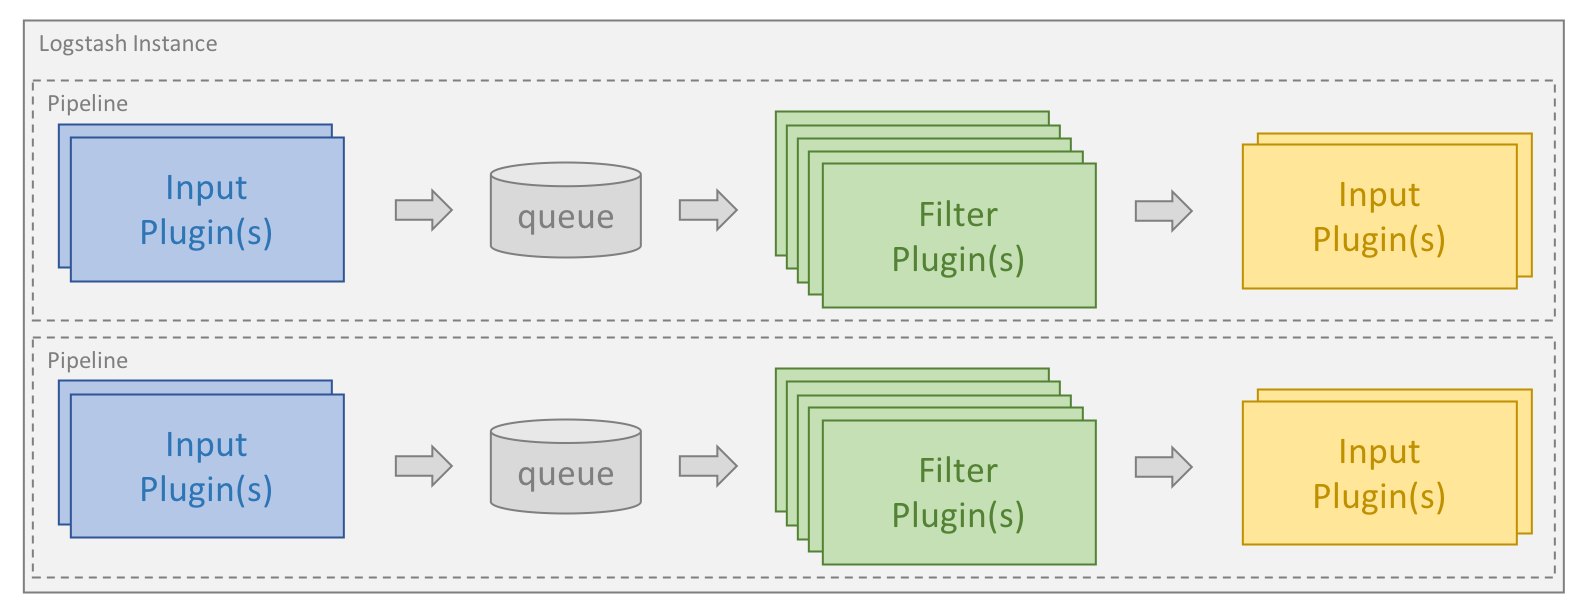
\includegraphics[width=0.5\linewidth]{./imagenes/logstash-pipeline.png}
  \caption{Logstash.}
  \label{fig:logstash}
\end{figure}

\subsection{Arquitectura de Logstash}\label{arquitectura-logtash}
Logstash es una herramienta para la administración de logs. Esta herramienta se puede utilizar para recolectar, parsear y guardar los logs para futuras búsquedas.La aplicación se encuentra basada en jRuby y requiere de Java Virtual Machine para correr. Como corre en JVM puede ser ejecutada en cualquier Sistema Operativo que corra JVM (Linux, Mac OS X, Windows).
En Logstash y con una infraestructura distribuida, cada servidor web debe ser configurado para correr Lumberjack (es opcional pero altamente recomendado para economizar recursos). Lumberjack hace un forward de los logs a un servidor corriendo Logstash con una entrada de Lumberjack. Como Lumberjack require SSL, los logs van a ser encriptados del servidor web al servidor de logs central.
Logstash is an open source, server-side data processing pipeline that ingests data from a multitude of sources simultaneously, transforms it, and then sends it to your favorite “stash.” (Ours is Elasticsearch, naturally.)	
Logstash soporta un número de entradas, códecs, filtros y salidas. Las entradas son las fuentes de datos. Los códecs esencialmente convierten un formato de entrada en un formato aceptado por Logstash, así como también transforman del formato de Logstash al formato deseado de salida. Estos son utilizados comúnmente si la fuente de datos no es una línea de texto plano. Los filtros son acciones que se utilizan para procesar en los eventos y permiten modificarlos o eliminar eventos luego de ser procesados. Finalmente, las salidas son los destinos donde los datos procesados deben ser derivados.
\section{Kibana}\label{kibana}
Kibana hace parte del grupo de aplicaciones liberadas por Elastic Search (Sharma, 2016)  para el análisis de datos a través de logs, comúnmente es conocido como “ELK Stack”, el cual refiere al uso de Elastic Search y Kibana en conjunto para la presentación y análisis de información a través de tableros de mando con estadísticas y series de tiempo.

\chapter{Arquitectura}

El sistema modular para la adquisición, gestión y visualización web de métricas de desempeño, está compuesto por cuatro capas cada una con una funcion especifica dentro de la representación y gestión de las métricas de desempeño que se presentan al usuario.

Los componentes del SMMD se clasifican de la siguiente manera:
\begin{enumerate}
	\item Recolectores de métricas
    \begin{enumerate}
    \item Collectd, un proceso que se ejecuta en segundo plano a nivel del nodo en donde se ejecutan los algoritmos o el procesamiento de datos, el cual se encarga de tomar todas las métricas de desempeño a través de plugins que se activan en un archivo de configuración.
    \item Metricbeat, un proceso que se ejecuta en segundo plano a nivel del nodo en donde se ejecutan los algoritmos o el procesamiento de datos el cual toma metricas básicas del sistema operativo y las envia al recolector de logs.
    \end{enumerate}
    \item Recolector de Logs
	\begin{enumerate}
      \item Logstash, es un proceso se ejecuta en el servidor, en este caso en el equipo que utiliza el investigador al cual los nodos envian la información de métricas de desempeño.
    \end{enumerate}
    \item Persistencia de Datos
    \begin{enumerate}
      \item Elastic Search, representa la capa de persistencia de datos y procesamiento, una vez la información ha sido recibida desde Logstash, elastic search se encarga de procesar y persistir la información en un formato de documento de typo JSON \footnote[1]{JavaScript Object Notation, un formato de intercambio de datos basado en el estándar ECMA-262 del lenguaje de programación Javascript}
    \end{enumerate}
    \item Presentación
    \begin{enumerate}
      \item Kibana, es un visualizador de datos, que permite explorar la información que se encuentra en Elastic Search y provee herramientas de fácil uso para la creación de paneles de control y vistas generales para la visualización de métricas de desempeño. Utiliza los paneles de control pre-definidos por metric beat para representar el uso de recursos tales como memoria, procesador y almacenamiento con actualizaciones en tiempo real.
    \end{enumerate}
\end{enumerate}

Tal como se puede observar en la figura \ref{fig:modelo-sistema} SMMD está modelado en una arquitectura de tipo cliente/servidor en donde el cliente está representado por los nodos que son asignados en el cluster al investigador para que este utilice sus recursos en la ejecución de programas o procesamiento de datos. El administrador provee de manera transparente al investigador dichos nodos con sistema operativo previamente instalado, que en el caso particular de este proyecto y acorde a los proyectos que se manejan actualmente en el CECAD, es un sistema operativo Linux en alguna de las dos distribuciones CentOS 7 o Ubuntu Xenial 16.04.
\\\\
Todo nodo que sea monitoreado utilizando SMMD, contiene dos colectores de métricas Collectd y Metric beat respectivamente los cuales envian información al servidor central, el cual está bajo el control de investigador y en donde se encuentran los componentes de recolección de logs, persistencia de datos y visualización. A partir de configuraciones específicas para el recolector de métricas Collectd, el investigador está en la capacidad de incluir diferentes plugins que le permitirán visualizar diferentes tipos de métricas de acuerdo a su necesidad particular. A nivel del servidor que como bien se menciono anteriormente está bajo el control del investigador, los componentes de recolección de logs, persistencia de datos y presentación, están aislados del sistema de archivos del sistema operativo y corren en un espacio de usuario alterno gracias al uso de contenedores Docker que están orquestados utilizando la herramienta docker-compose\footnote{https://docs.docker.com/compose, Compose es una herramienta para definir y correr aplicaciones de múltiples contenedores en Docker}, los cuales no tienen dependencia directa las librerias o software del sistema operativo permitiendo así la operabilidad en distintos sistemas operativos que soporten la tecnología Docker, tales como MacOS, Windows y Linux en distintas arquitecturas de procesador como los son x86, amd64, ARM, ppc64le (IBM Power) y s390x (IBM Z). Adicionalmente como consecuencia de la independencia de estos componentes con librerias propias del sistema operativo, permite que la instalación sea mucho más sencilla para el investigador sin la necesidad que este tenga que preocuparse por instalar dependecias en su sistema, con la simple instalación de Docker el investigador tendrá a su disposición el componente del servidor sin inconveniente alguno.

A continuación de presentará en detalle cada uno de los componentes de las capas de SMMD en donde se mencionará en detalle la interoperatibilidad entre dichas tecnologías que permite el funcionamiento de SSMD.

\begin{figure}
 \centering
  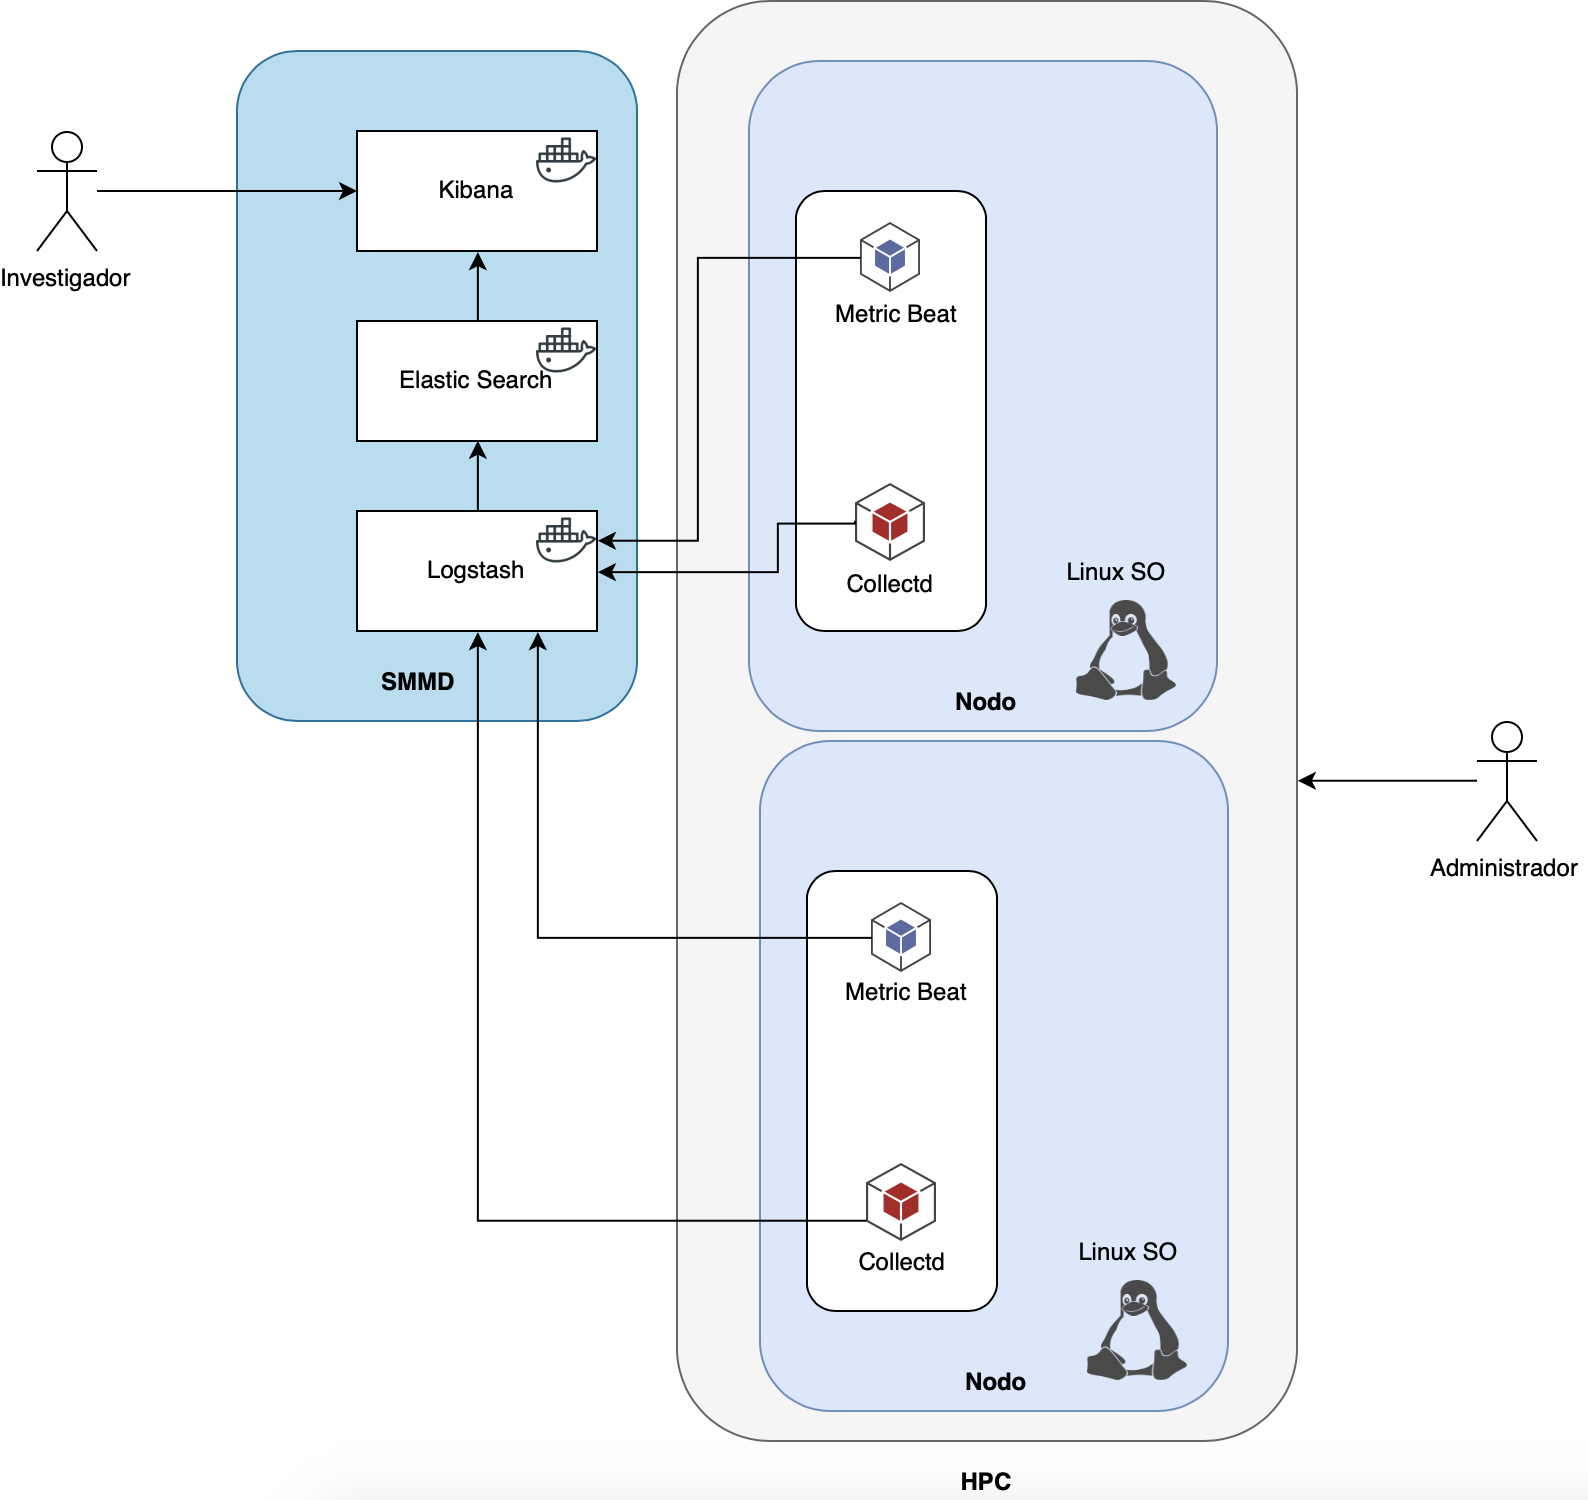
\includegraphics[width=0.9\linewidth]{./imagenes/arquitectura-general.png}
  \caption{Modelo General del Sistema SMMD.}
  \label{fig:modelo-sistema}
\end{figure}


\newpage

\section{Recolección de Métricas}



\subsection{Tipos de Métricas}

En el espacio del tipo de métricas que SMMD soporta actualemente se suman los dos grandes conjuntos de métricas que provee el sistema a través de las herramientas Metricbeat y Collectd, cada uno es una tecnología separada e independiente con propositos e implementación complementamente distintos los cuales se describen a continuación.

Las métricas soportadas son 


\subsection{Metricbeat}\label{metricbeat}
Metricbeat\footnote[1]{https://www.elastic.co/products/beats/metricbeat} conocido también como Elastic Metricbeat, hace parte de la suite de herramientas de Elastic\footnote[2]{Elastic NV, compañía Europea fundada por Shay Banon en 2012 conocida antiguamente como Elasticsearch, es una una compañía dedicada a ofrecer servicios de tipo SaaS (Software como servicio) para el análisis y búsqueda de logs principalmente, servicios usados por compañías reconocidas como: eBay, Cisco, Microsoft y la NASA).} es un software que corre como servicio o demonio el cual permite procesar métricas de desempeño básicas como: uso de CPU, carga promedio del sistema, memoria, uso de red y lecto-escritura en disco. 
Provee la capacidad de habilitar módulos para procesar métricas de otros sistemas como HAProxy, Apache Kafka, Kubernetes, MongoDB, MySQL entre otros. Debido a que su instalación es muy sencilla y su integración con otros productos de la misma compañía es buena, es la opción estandar para la obtención de métricas básicas de desempeño.



\subsection{Collectd}\label{demonio-collectd}
Existen diversos tipos de software para la recolección de métricas de desempeño, para el caso particular de este proyecto se utilizará \textbf{Collectd}, un software de tipo demonio\footnote[3]{Un programa de computadora que corre como un proceso en segundo plano el cual no está bajo el control directo del usuario actual del sistema}, 

\subsection{Statsd}\label{statsd}
Statsd es un demonio de muy facil uso



\section{Gestión de Métricas}
Logstash es un motor de procesamiento y recopilación de datos basado en plugins. Incluye una gran variedad de plugins que permiten configurarlo fácilmente para recopilar, procesar y reenviar datos en muchas arquitecturas diferentes. \hl{Registrar fuente y actualizar}

El procesamiento se organiza en uno o más pipelines. En cada pipeline, uno o más plugins de entrada reciben o recopilan datos que luego se colocan en una cola interna. De manera predeterminada, esta es pequeña y se almacena en la memoria, pero puede configurarse para ser más amplia y permanecer en el disco para mejorar la confiabilidad y la persistencia.

Los hilos de procesamiento leen datos de la cola y los procesan a través de cualquier plugin de filtro configurado en secuencia. Logstash viene de fábrica con una gran cantidad de plugins destinados a tipos específicos de procesamiento, y así es como se analizan, procesan y enriquecen los datos.

Una vez que se procesan los datos, los hilos de procesamiento envían los datos a los plugins de salida correspondientes, que son los responsables de formatear y enviar los datos hacia adelante, por. ej., a Elasticsearch.

Los plugins de entrada y salida también pueden tener un plugin de códec configurado. Esto permite formatear datos antes de colocarlos en la cola interna o antes de enviarlos a un plugin de salida.


\section{Persistencia}
Elasticsearch es un motor de búsqueda basado en Lucene. Lucene es una API gratuita y de código abierto para hallar informaciones y se usa mucho para crear motores de búsqueda.

Elasticsearch, a través de interfaces web HTTP y documentos JSON, permite interactuar de forma sencilla con su núcleo y realizar búsquedas de texto completo muy eficaces.

La misión de Elasticsearch parte de una convicción de Shay Banon, el fundador: “Search is something that any application should have”. Basándose en este credo, Banon trabajó durante años para llevar su compañía a la cima de la escena informática mundial.

Hoy Elasticsearch es un sistema distribuido que escala horizontalmente, basado en nodos que a su vez se dividen en clústeres. La comunicación hacia y desde los clústeres se realiza a través de las REST API que utilizan HTTP. Las aplicaciones de los clientes que utilizan este proyecto se pueden escribir en cualquier lenguaje. La arquitectura subyacente es obviamente invisible para el usuario, que percibe todo como una entidad única, aunque la naturaleza distribuida de la pila hace que los procesos se interconecten entre sí a través de un intercambio continuo de mensajes entre los nodos. Estos últimos tienen tareas muy específicas que se dividen en autonomía, dependiendo de las configuraciones que se le da a los distintos balances de carga. Si los recursos establecidos al principio no son suficientes, Elasticsearch puede “ampliar” su capacidad de procesamiento activando nuevos nodos y creando nuevos clústeres, con total autonomía; de aquí su naturaleza escalable.
 
\newpage

\section{Comunicación}

\section{Protocolos de operabilidad}
Aqui que protocolo utiliza logstash, collectd y metric beat.


\subsection{Operabilidad en Red}
En el aspecto de la comunicación entre cliente y servidor, SMMD permite dos configuraciones básicas como se puede observar en la figura \ref{fig:modelo-comunicacion} 

\begin{enumerate}
	\item Usuario externo: En este escenario el investigador se encuentra en un red externa fuera del rango IPs accesible necesario para que las másquinas virtuales asignadas por el administrador envien información periodica al servidor. La linea roja en el diagrama \ref{fig:modelo-comunicacion} representa el flujo de la información desde el interior de la red del centro de computo hasta el servidor principal SMMD controlado por el investigador. Para este escenario, el investigador deberá solicitar al administrador del HPC acceso a la red interna a través de un VPN con el fin de establecer una LAN virtual entre los nodos asignados en el cluster y el equipo servidor que recibira el reporte de las métricas de desempeño.
	\item Usuario interno: En este escenario el usuario se encuentra físicamente en la LAN del centro de computo, y comparte una misma subred lo cual hace que los nodos asignados vean la dirección ip del servidor y puedan enviar la información de métricas de desempeño.
\end{enumerate}
Como se mencionará en el capítulo de instalación, los valores de red a configurar en los nodos son dinámicos y permiten ajustarse a cualquier de los dos escenarios mencionados anteriormente.

\begin{figure}[h]
 \centering
  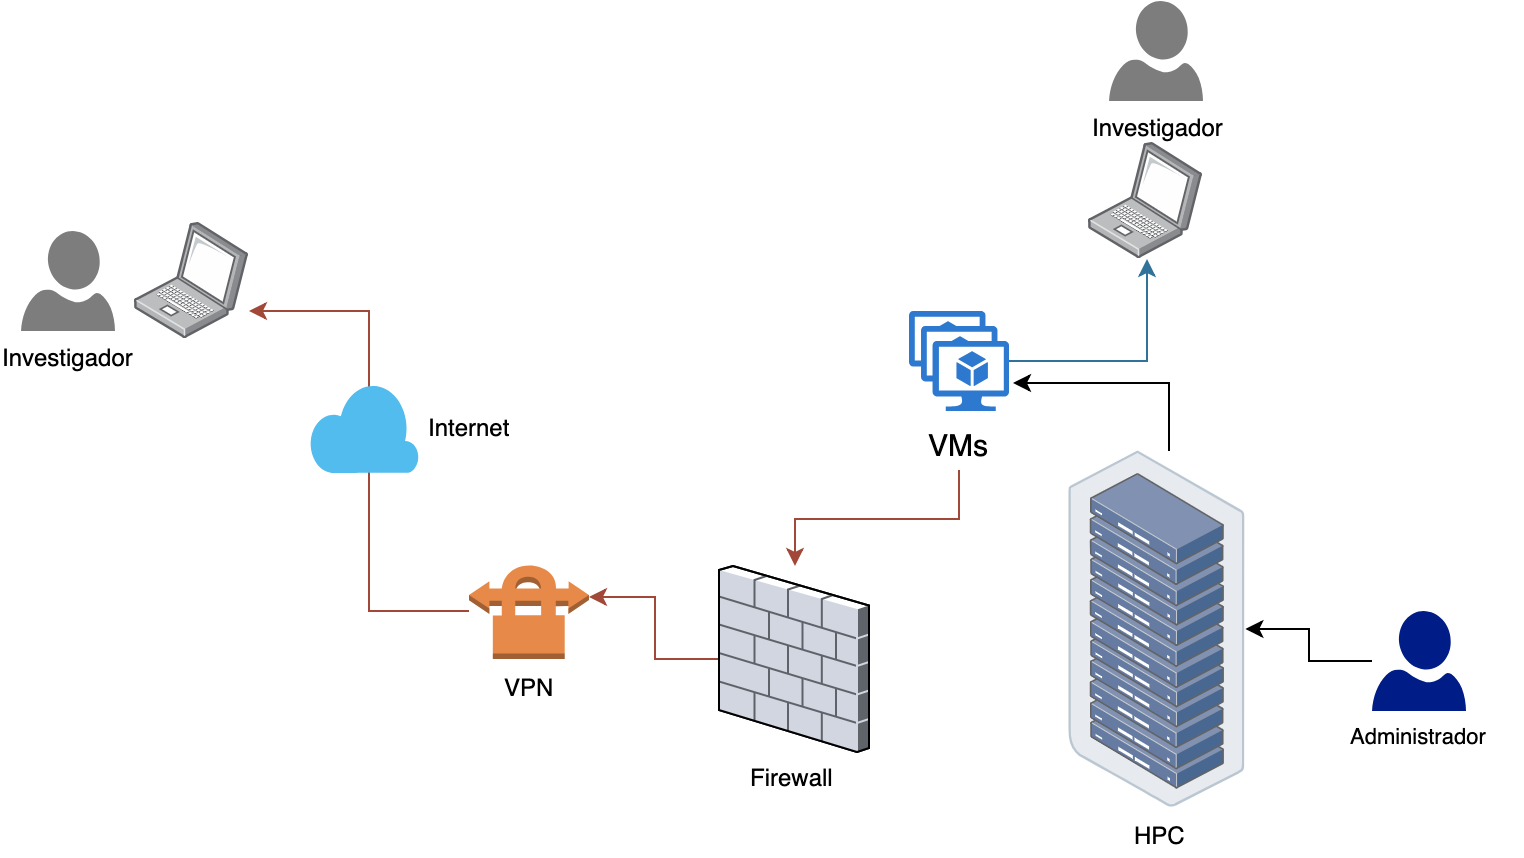
\includegraphics[width=0.9\linewidth]{./imagenes/comunicacion.png}
  \caption{Comunicacion Cliente - Servidor.}
  \label{fig:modelo-comunicacion}
\end{figure}
\newpage
\section{Visualización}
Kibana es una plataforma de análisis y visualización de código abierto diseñada para trabajar con Elasticsearch. Utiliza Kibana para buscar, ver e interactuar con datos almacenados en los índices de Elasticsearch. Puede realizar análisis de datos avanzados y visualizar fácilmente sus datos en una variedad de gráficos, tablas y mapas.

Kibana facilita la comprensión de grandes volúmenes de datos. Su sencilla interfaz basada en navegador le permite crear y compartir rápidamente paneles dinámicos que muestran cambios en las consultas de Elasticsearch en tiempo real.

La configuración de Kibana es muy fácil. Puedes instalar Kibana y comenzar a explorar sus índices Elasticsearch en minutos - sin código, sin infraestructura adicional requerida.


\chapter{Implementación de SMMD}

A continuación de describe la estructura de la implementación del Sistema Modular de métricas de desempeño en el CECAD.
Se describe una arquitectura de tipo cliente/servidor, donde el servidor es el equipo del investigador, y los clientes son los nodos
que le han sido asignados para trabajar dentro del centro de computación de alto desempeño.


\subsection{Requisitos mínimos del sistema}
Para hacer uso de SSMD el sistema operativo deberá tener los siguientes requerimientos minímos para poder ser instalado y utilizado.
Estos requisitos se dividen en requisitos del servidor y cliente.

\subsubsection{Requisitos del Servidor}
Los siguientes son los requisitos de software para instalar el software servidor de SSMD.

\begin{enumerate}
	\item Docker Community Edition. Disponible para su descarga en \url{https://docs.docker.com/install}
	\item Python 2.7. Disponible para su descarga en \url{https://www.python.org/downloads/}
	\item Ansible. Ver \url{https://docs.ansible.com/ansible/latest/installation_guide/intro_installation.html}
	\item Requisitos opcionales 
	\begin{itemize}
		\item Virtualbox \url{https://www.virtualbox.org/wiki/Downloadsre}
		\item Vagrant \url{https://www.vagrantup.com/downloads.html}
	\end{itemize}
\end{enumerate}

\subsubsection{Requisitos del Cliente}
Los siguientes son los requisitos de software para instalar el software servidor de SSMD.
\begin{enumerate}
	\item Python 2.7. Disponible para su descarga en \url{https://www.python.org/downloads/}
	\item Acceso SSH habilitado para conexiones salientes.
    \item Sistema Operativo CentOS 7 o Ubuntu 16.04 LTS (Xenial Xersus) 
    \begin{itemize}
    	\item CentosOS: \url{https://www.centos.org/download/}
    	\item Ubuntu: \url{http://releases.ubuntu.com/16.04/}
    \end{itemize}
\end{enumerate}


\section{Fuentes de Instalación}\label{fuentes-instalacion}
El código fuente de este proyecto se encuentra en el repositorio público \url{https://github.com/bizoru/ssmd}, este puede ser descargado desde cualquier lugar 
y está disponible con uso de licencia GNU GPL v3.\footnote{Licencia Pública General GNU https://www.gnu.org/licenses/gpl-3.0.en.html}
\\\\
La estructura del código se puede visualizar en la Figura \ref{fig:estructura-fuente}

\begin{figure}[h]
 \centering
  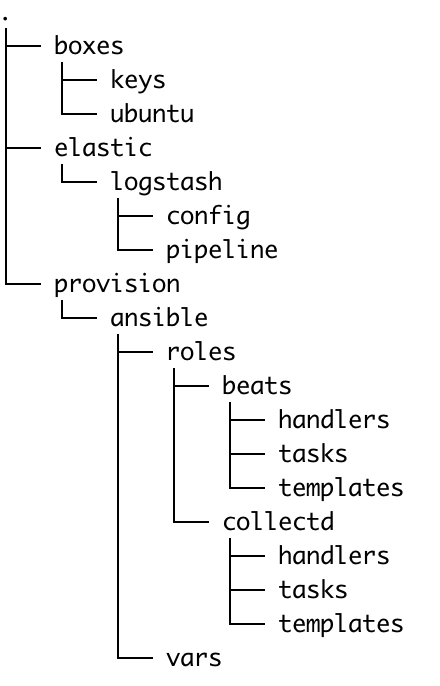
\includegraphics[width=0.3\linewidth]{./imagenes/estructura-fuente.png}
  \caption{Instalación de SMMD en Nodos Cliente.}
  \label{fig:estructura-fuente}
\end{figure}

A continuación se describe la estructura de archivos que se encuentran en el código fuente de acuerdo con su funcionalidad y propósito.

\newpage

Las carpetas que se encuentran en el código fuente de acuerdo con la figura \ref{fig:estructura-fuente} son:

\begin{itemize}
	\item boxes
    \begin{itemize}
      \item[] Esta carpeta contiene las imágenes de \gls{vagrant} para hacer la demostración de SMMD sin necesidad de tener nodos externos. Contiene las llaves SSH \footnote{SSH, Secure Shell, Protocolo para operar computadoras a través de la red de manera segura.} que se utilizarán para acceder a los nodos y la definición de los mismos.
    \end{itemize}
    \item elastic
    \begin{itemize}
      \item[] Esta carpeta contiene el archivo principal de \gls{docker_compose} el cual contiene las imágenes de Logstash, Kibana, y Elastic Search, aquí se encuentra toda la configuración de puertos, nombre del cluster y contraseña de acceso para el sistema de SMMD a través de Kibana.
    \end{itemize}
    \item provision
    \begin{itemize}
      \item[] Esta carpeta contiene los scripts\footnote{Conjunto de \gls{script}s que permite la automatización de procesos.} de aprovisionamiento, allí se encuentran dividos en unidades lógicas llamados roles, estos definen que componente del cliente se va a instalar, para este caso, el demonio Collectd (Ver sección \ref{demonio-collectd}) y MetricBeat (Ver sección \ref{metricbeat}). También encontramos la definición de las variables de cada uno de los programas a instalar, y las configuraciones especificas tanto para Collectd como para metricbeat.
    \end{itemize}
\end{itemize}

\section{Instalación}
La instalación de SMMD consta de dos etapas: La primera etapa consiste en la descarga de la fuente de instalación, (Ver sección \ref{fuentes-instalacion}) preparar los requisitos
de instalación del servidor de acuerdo al sistema operativo del investigador, posteriormente se deben subir los servicios de Logstash (Ver sección \ref{logstash-description}), Elastic Search (Ver sección \ref{elastic-search} ) y Kibana (Ver sección \ref{kibana}).

\subsection{Instalación del Servidor SMMD}
Es importante tener en cuenta los siguientes puntos en consideración para que el proceso de instalación del servidor se pueda realizar a cabo sin problema:
\begin{enumerate}
	\item Habilitar las reglas de firewall para que pueda tener comunicación con los diferentes nodos.
\end{enumerate}
Para proceder con la iniciación de los servicios de Kibana, ElasticSearch y Logstash realice los siguientes pasos:

\begin{enumerate}
	\item Ingrese a la carpeta \texttt{elastic}
	\item Ejecute el comando \texttt{docker-compose up}
\end{enumerate}

\begin{figure}[h]
 \centering
  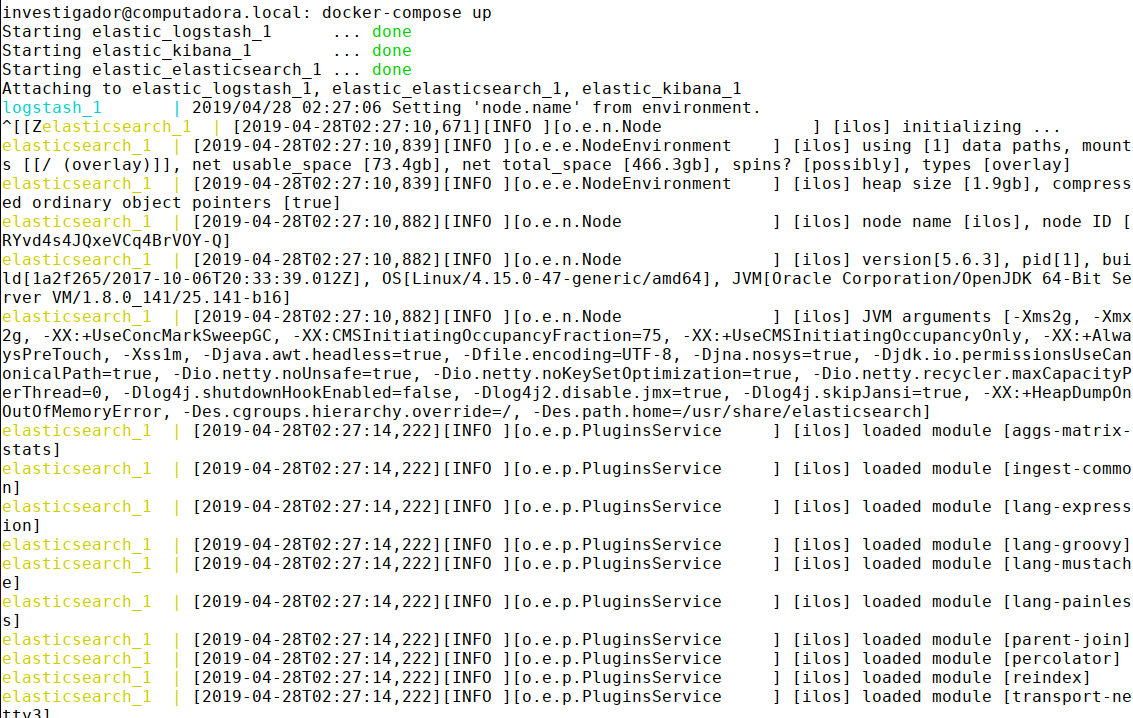
\includegraphics[width=0.85\linewidth]{./imagenes/docker-compose-up.png}
  \caption{Ejemplo, resultado de la ejecución de docker-compose up, iniciación de servicios}
  \label{fig:docker-compose-up}
\end{figure}

El proceso tomará algun tiempo en completarse una vez esta haya finalizado podrá acceder la interfaz de administración ingresando a \url{http://localhost:5601}, el usuario es \textit{elastic} y la contraseña es \textit{changeme}.

\begin{figure}[h]
 \centering
  
\includegraphics[width=0.4\linewidth]{./imagenes/login-page.png}
  \caption{Pantalla de inicio de sesión en Kibana}
  \label{fig:kibana-login-page}
\end{figure}

Con estos pasos se ha completado la instalación del servidor central donde el investigador podrá acceder al panel de administración y visualizar las métricas de desempeño.

\newpage
\subsection{Aprovisionamiento de Nodos}
SMMD provee una herramienta para hacer la instalación de Metricbeat y collectd, a través de un script de aprovisionamiento dicho script establecerá una conexión SSH hacia los nodos en el cluster y utilizando Ansible hará la instalación del software requerido y configurará los valores necesarios para la comunicación con el servidor central.

\begin{figure}[ht]
 \centering
  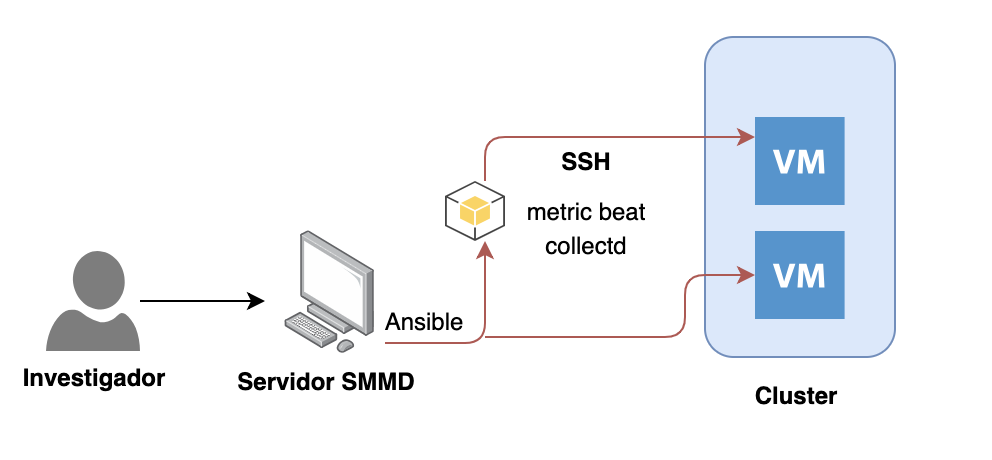
\includegraphics[width=0.5\linewidth]{./imagenes/modelo-instalacion.png}
  \caption{Instalación de SMMD en Nodos Cliente.}
  \label{fig:modelo-instalacion}
\end{figure}

Las siguientes son consideraciones importantes ha tener en cuenta para aprovisionar los nodos que enviarán las métricas de desempeño al nodo central.
\begin{enumerate}
	\item El servidor SMMD deberá estar en la misma red en la que están los nodos, con el fin de poder recibir las métricas de desempeño a través de la red.
	\item Cada nodo deberá tener una llave de acceso \gls{ssh} en el archivo \texttt{./ssh/authorized\_keys} con un usuario con permisos de administración.
	\item Habilitar el usuario super administrador y llaves SSH
	\item Habilitar reglas de firewall para habilitar comunicación externa con el servidor central.
	\item Configuración especial en métricas de collectd que se requieran para utilizar en Elastic Search.
\end{enumerate}

Como se puede ver en la figura \ref{fig:modelo-instalacion} el investigador ejecuta el código de aprovisionamiento de \gls{ansible} y este se encarga de hacer la instalación de los paquetes collectd y metricbeat en los nodos o máquinas virtuales que le han sido asignadas en el cluster HPC.

\newpage

El proceso de aprovisionamiento utiliza el script que se encuentra en la ruta \texttt{/provision/provision.sh}, este script se ejecuta de la siguiente manera:

\begin{verbatim}
     export ELASTIC_SEARCH_SERVER=<ip>
     export LOGSTASH_SERVER=<ip>
     provision.sh <host>
\end{verbatim}

Donde las variables para \texttt{ELASTIC\_SEARCH\_SERVER} y \texttt{LOGSTASH\_SERVER} en el campo de \texttt{ip} debe asignarse el valor de la ip pública del servidor en el cual se está ejecutando el script de aprovisionamiento.

\begin{figure}[h]
 \centering
  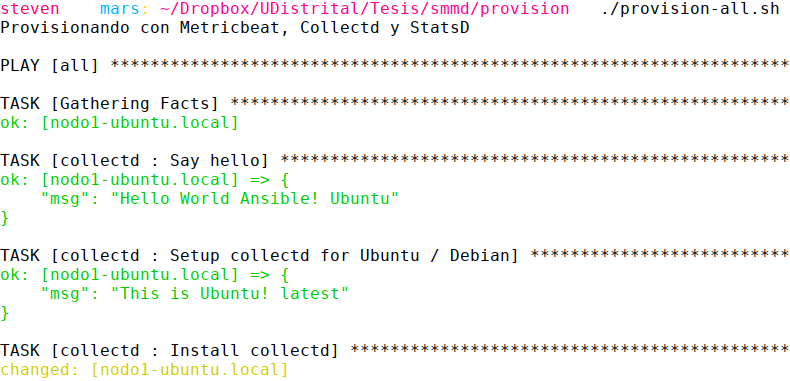
\includegraphics[width=0.6\linewidth]{./imagenes/provision_all.png}
  \caption{Aprovisionamiento de SMMD en los nodos cliente.}
  \label{fig:aprovisionamiento-nodos}
\end{figure}
Como se puede ver en la figura \ref{fig:aprovisionamiento-nodos} este es el resultado que entrega la consola en el momento de ejecutar el aprovisionamiento, al final del proceso, todos los nodos que hayan sido provisionados, tendrán activos los servicios de metricbeat, collectd y statsd.
\clearpage

\section{Uso}
A continuación se describe el uso de SMMD
\subsection{Visualización de Métricas de Desempeño}
asdf
Seleccionar las métricas de desempeño de cada nodo según el nombre de host asignado.
\begin{figure}[h]
 \centering
  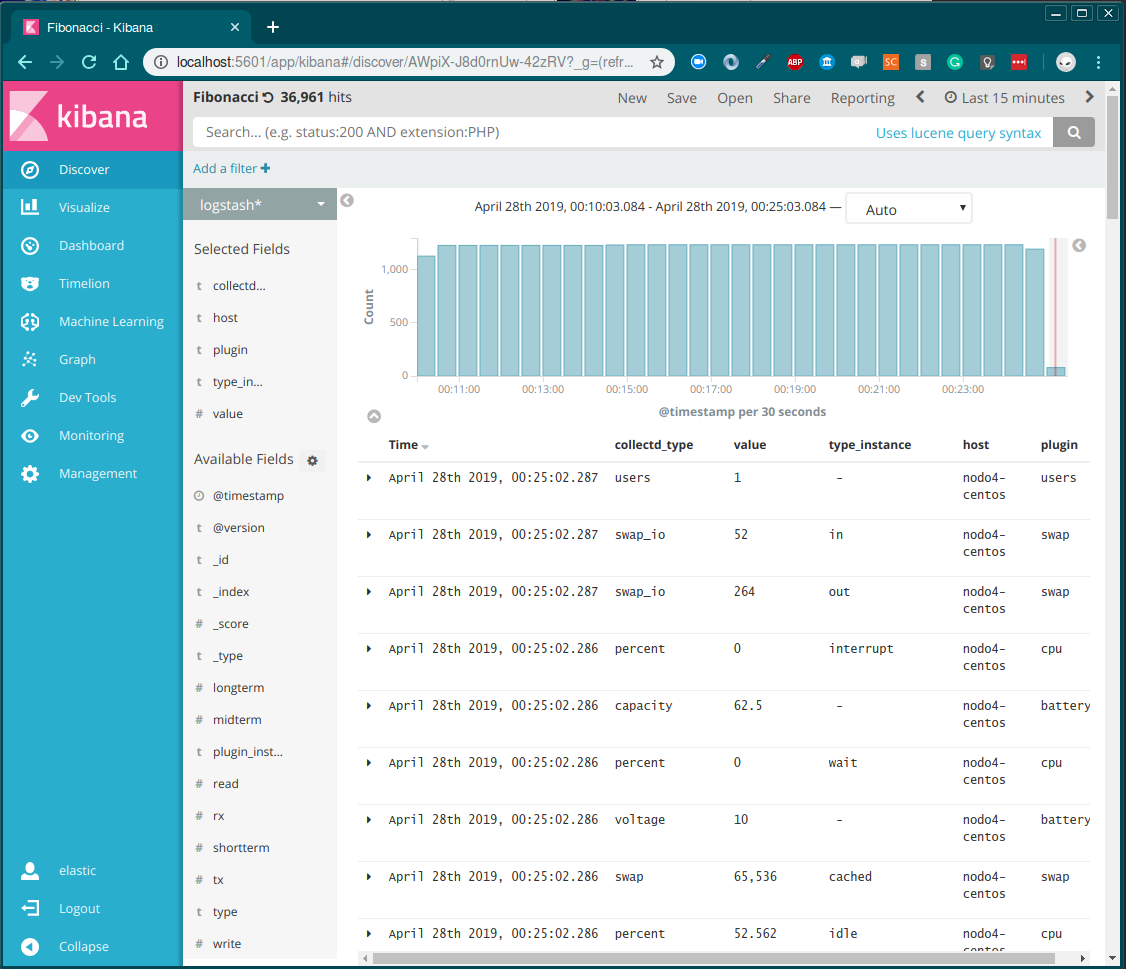
\includegraphics[width=0.6\linewidth]{./imagenes/kibana-home.png}
  \caption{Pantalla Principal de SMMD}
  \label{fig:home-smmd}
\end{figure}

\newpage

\subsection{Ajustes generales}
Ajustes generales a nivel del motor de base de datos no relacional Elastic Seach para el almacenamiento de la información de las métricas de desempeño.


\subsection{Plugins}

Ajustes generales a nivel de plugin del lado del cliente. Inclusión de nuevas métricas y valores especificos en la configuración del demonio collectd.





\chapter{Evaluación de SMMD}

Una vez instalada la apliacion de SMMD en el CECAD se mostrará a continuación sus funcionalidades principales y su manejo.

\subsection{Caso práctico CECAD}

En la figura se puede observar la creación de un dashboard personalizado el cual muestra los valores de las métricas \texttt{fibonacci-count},\texttt{fibonacci-average},\texttt{fibonacci-sum}, valores que son enviados a través de la libreria cliente de statsd en python.


\begin{figure}[h]
 \centering
  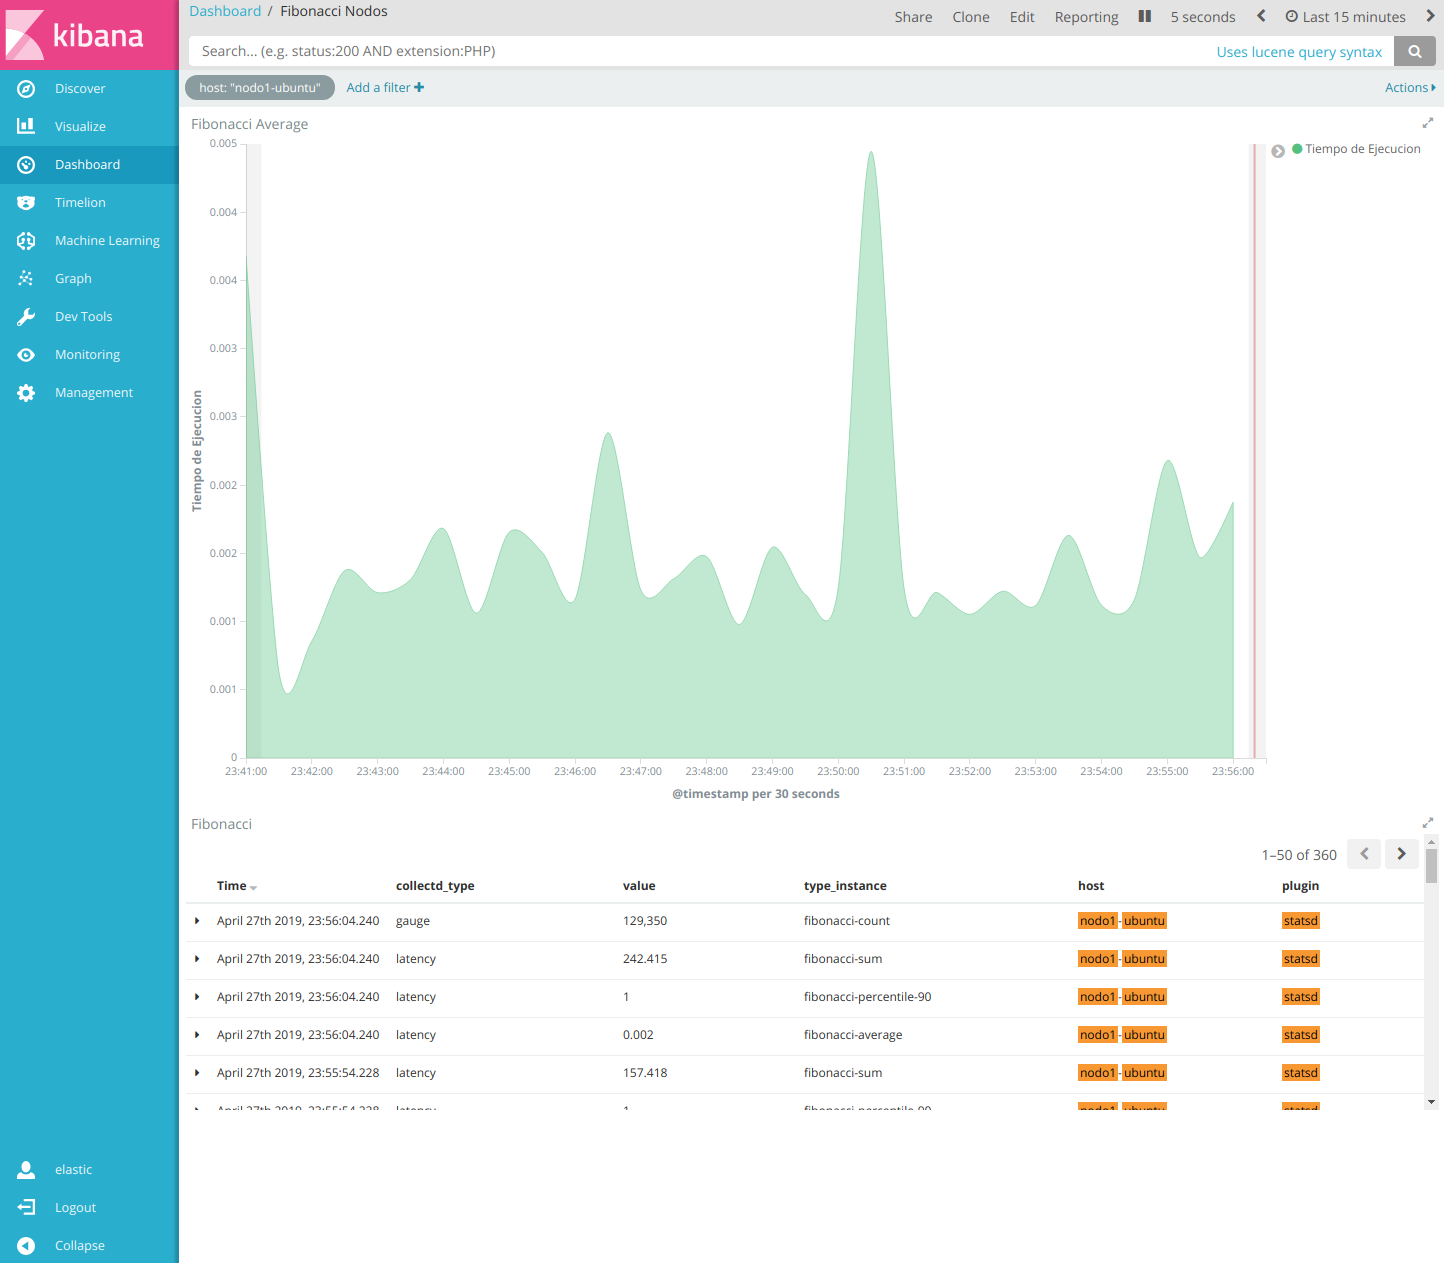
\includegraphics[width=0.8\linewidth]{./imagenes/dashboard-fibonacci.png}
  \caption{Dashboard Personalizado para la medición de métricas recibidas por StatsD}
  \label{fig:dashboard-fibonacci}
\end{figure}
\chapter{Conclusiones}
\chapter{Principales aportes y divulgación}
\chapter{Recomendaciones y Futuros Trabajos}

\section{tal}
asdfasdfdasf
adsf
asdf
adsf
ads
fdas
fdas
a
sdf
\printglossaries
\bibliographystyle{apacite}
\bibliography{referencias/indice}
\end{document}